
\section{Calculating b-value, BVALUE}

\index{B-value}\index{BVALUE}

BVALUE is a program to make b-value plots using a NORDIC input file (also compact). A postscript plot file is generated. 

The questions are: 

\verbatiminput{include/bvalue.run}
\index{Maximum likelihood b-value} 
\index{Bvalue.out}
\index{Bvalue.eps}

The output file bvalue.out contains the same information in the same format as shown in the example above. The file can be used with other plotting programs to make 'nicer looking' b-value plots. An example is shown in Figure \ref{fig:b-value}. 

\begin{figure}
\htmlimage{scale=2.0}
\centerline{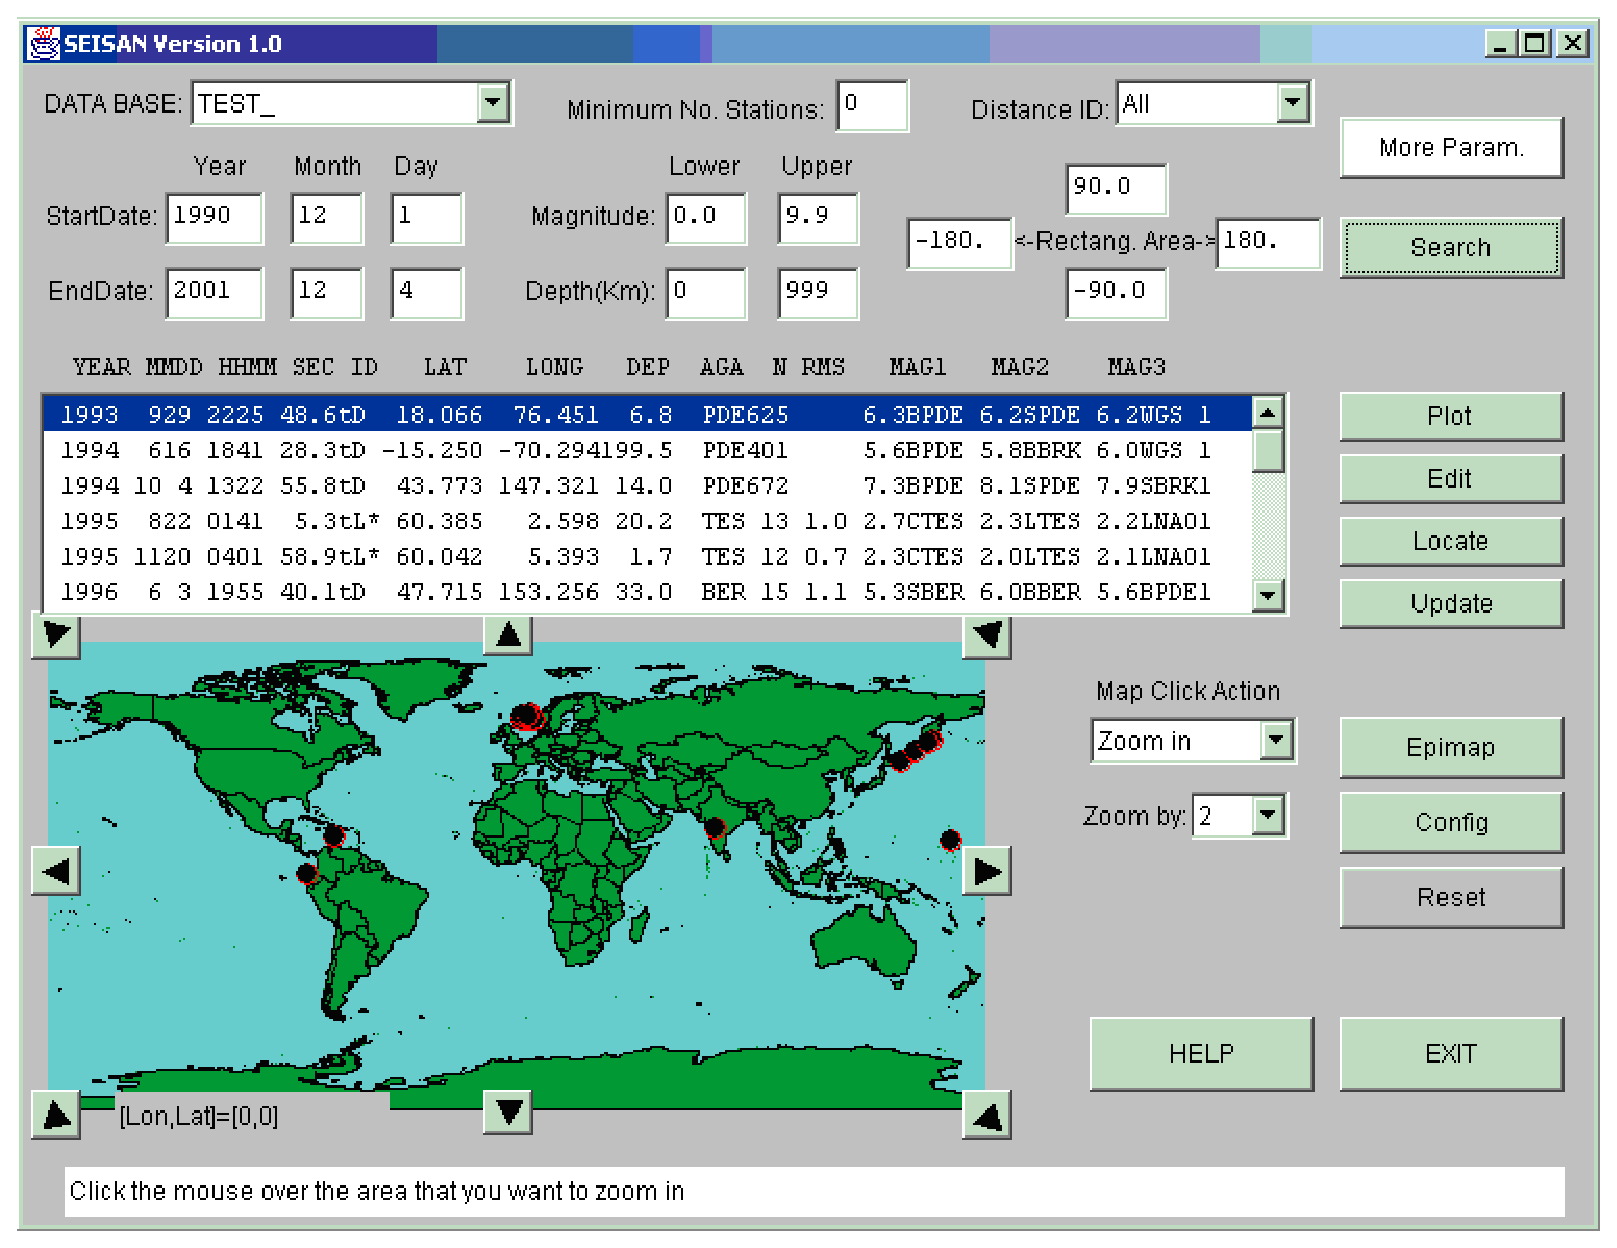
\includegraphics[width=0.9\linewidth]{fig2/fig6}}
\caption{
An example of a b-value plot. The bars are number of events and crosses the accumulated number of events. 
}
\label{fig:b-value}
\end{figure}


